\begin{frame}{Introduction}
\begin{itemize}
\item What is Ceph?
\item Why we are looking at it?
\item File Storage Vs Object Storage
\end{itemize}
\end{frame}
\note{I am going to cover in the introduction, What is Ceph, Why are we looking at it, What is a File and Object store including their differences.}
\begin{frame}{Introduction - What is Ceph}
\begin{figure}[h]
    \centering
    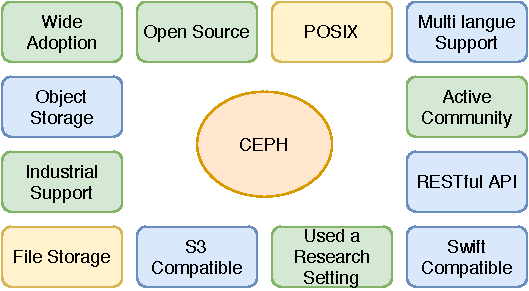
\includegraphics[width=\linewidth]{img/what-is-ceph.pdf}
\end{figure}
\note{So Ceph is essence is Open Source scale-able distributed storage platform, that be used as a POSIX File System, Object store or Block device. It is S3 and Swift Compatible and has a a restful API that is implemented in multiple languages including Python,C++ and Java. It is approximately 14 years old and started as PhD project however has since been acquired by Redhat. It has many industrial and research facilities that use it, including STFC, CERN, OCADO and BLOOMBERG}
\end{frame}{}

\begin{frame}{Introduction - File Storage}

\begin{columns}
    \begin{column}{0.47\textwidth}
    \begin{block}{File Storage}
        \begin{itemize}
            \item Stores data in  Hierarchical structure
            \item 
            \item GPFS, BeeGFS, CephFS,
            
        \end{itemize}
    \end{block}
    \end{column}
    \begin{column}{0.47\textwidth}
        \begin{figure}
        \centering
        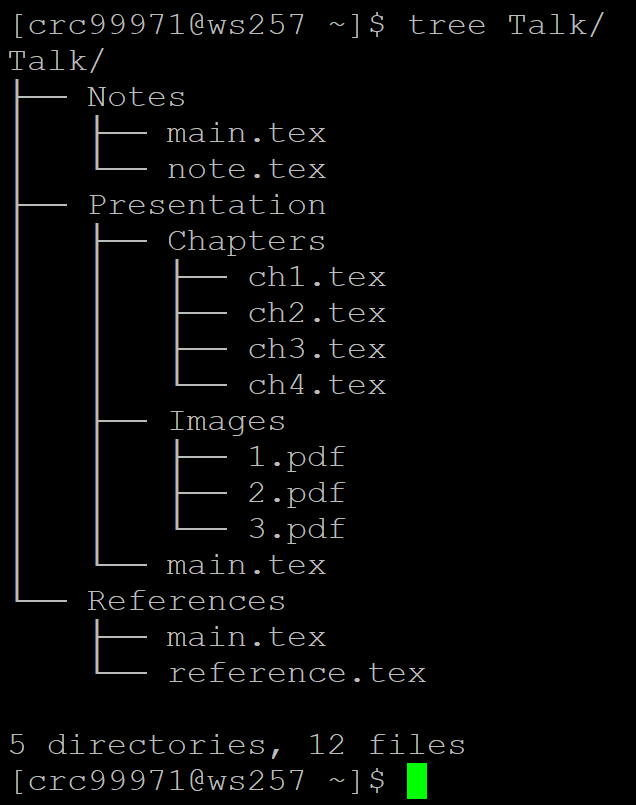
\includegraphics[width=\textwidth,height=0.7\textheight,keepaspectratio]{img/tree.PNG}
        \caption{File Storage}
        \label{fig:my_label}
    \end{figure}
    \end{column}
\end{columns}
\end{frame}
\begin{frame}{Introduction - Object Storage}
    \begin{figure}
        \centering
        \includegraphics[width=\textwidth,height=0.7\textheight,keepaspectratio]{img/imagetree.PNG}
        \caption{Image Folder}
        \label{fig:my_label}
    \end{figure}  
\end{frame}


\begin{frame}{Introduction - Storing Images}
\begin{columns}
    \begin{column}{0.47\textwidth}
    \begin{figure}
        \centering
        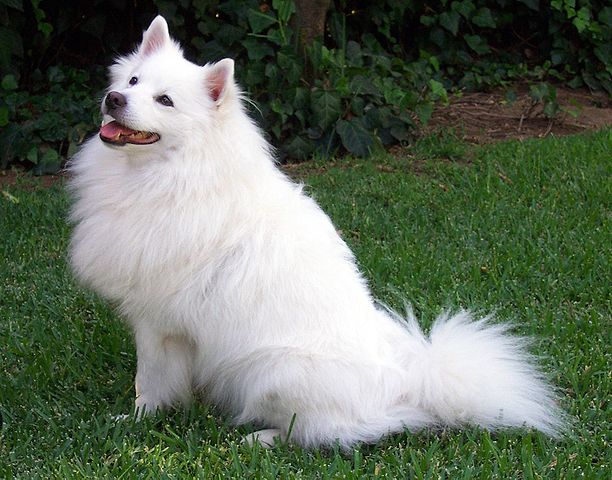
\includegraphics[width=\textwidth,height=0.45\textheight,keepaspectratio]{img/dog.jpg}
        \label{fig:my_label}
    \end{figure}
    \end{column}
    \begin{column}{0.47\textwidth}
    \begin{figure}
        \centering
        \includegraphics[width=\textwidth,height=0.55\textheight,keepaspectratio]{img/imagetree.PNG}
        \label{fig:my_label}
    \end{figure}
    \end{column}
\end{columns} 
\begin{block}{Where to store}
\begin{description}
    \item [A] Images/Animals/Dogs
    \item [B] Images/Animals/Cats
    \item [C] Images/Landscapes/Urban
\end{description}
\end{block}
\end{frame}
\note{If we have a file-system for storing images, that has subdirectories, Landscapes and Animals, and say Landscapes has subdirectories of Coastal, Mountain, Urban, etc. and Animals has subdirectories of; Fish, Dogs, Cats, etc. Now if we have well-defined images, of just Dogs, Coasts, Mountains and Cats. This system works perfectly well.}
\begin{frame}{Introduction - Storing Images}
\begin{columns}
    \begin{column}{0.47\textwidth}
    \begin{figure}
        \centering
        \includegraphics[width=\textwidth,height=0.45\textheight,keepaspectratio]{img/dogorbeach.jpg}
        \label{fig:my_label}
    \end{figure}
    \end{column}
    \begin{column}{0.47\textwidth}
    \begin{figure}
        \centering
        \includegraphics[width=\textwidth,height=0.55\textheight,keepaspectratio]{img/imagetree.PNG}
        \label{fig:my_label}
    \end{figure}
    \end{column}
\end{columns} 
\begin{block}{Where to store}
\begin{description}
    \item [A] Images/Animals/Dogs
    \item [B] Images/Landscapes/Coastal
    \item [C] Images/Landscapes/Urban
\end{description}
\end{block}
\end{frame}
\note{However, if we have an image of a Dog at the Beach, where do you place this image within this structure. It could either go in the Dogs or Coastal directory either would make sense. However, when looking for that image again, are you going to have remembered where you put it. Object Storage would make sense here as the data doesn't have an inherent structure as much as we can try.}

\begin{frame}{Object Storage}
    \begin{columns}
    \begin{column}{0.47\textwidth}
    \begin{figure}
        \centering
        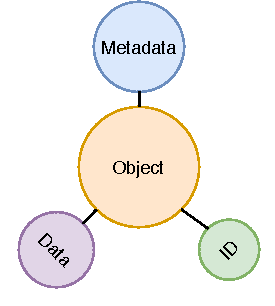
\includegraphics{img/object.pdf}
        \caption{Object}
        \label{fig:my_label}
    \end{figure}
    \end{column}
    \begin{column}{0.47\textwidth}
    \begin{figure}
        \centering
        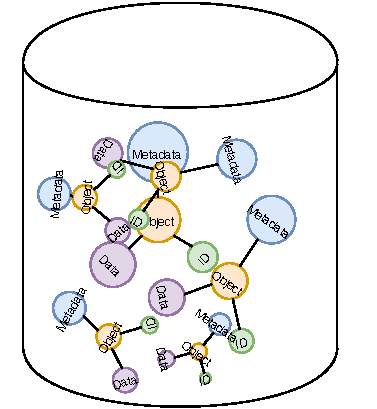
\includegraphics[width=\textwidth,height=0.55\textheight,keepaspectratio]{img/pool.pdf}
        \caption{Image Pool}
        \label{fig:my_label}
    \end{figure}
    \end{column}
\end{columns}
\end{frame}
\note{Instead, we can have a Pool called images and place the images inside that pool as objects, with metadata attached identifying what the image is instead.  Now we can just put images in the pool without having to worry where to put them. And when we want to get the image with a Dog at the Beach, we can look through the metadata and find images with that included that information. }
\begin{frame}{Introduction - Object Storage}
\begin{columns}
    \begin{column}{0.47\textwidth}
    \begin{block}{Object Storage}
        \begin{itemize}
            \item Stores data in  flat structure
            \item Good for unstructured data
            \item Flexible data size, very small/very Large
        \end{itemize}
    \end{block}
    \end{column}
    \begin{column}{0.47\textwidth}
    \begin{figure}
        \centering
        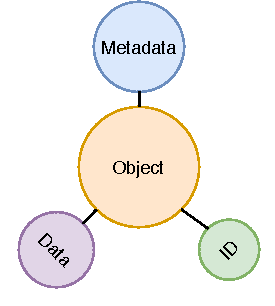
\includegraphics{img/object.pdf}
        \caption{Object Structure}
        \label{fig:my_label}
    \end{figure}
    \end{column}
\end{columns}
\end{frame}